% !TEX encoding = UTF-8
% !TEX TS-program = pdflatex
% !TEX root = ../tesi.tex

%**************************************************************
\chapter{Resoconto Stage}
\label{cap:resoconto-stage}
%**************************************************************

%**************************************************************
\section{Pianificazione}
\subsection{Pianificazione iniziale}\label{sec:pianificazione-iniziale}
Una prima pianificazione delle attività è stata fatta da me insieme al tutor aziendale, prima dell'inizio dello stage, principalmente definendo il Piano di Lavoro, documento necessario per iniziare lo stage e per avere un'idea delle tempistiche necessarie al completamento degli obiettivi discussi. Durante lo svolgimento dello stage tuttavia, la pianificazione originaria ha subito delle piccole modifiche, in quanto alcune attività hanno richiesto più tempo di altre. 

\subsection{Sistema di Issue e Gantt}
Per essere sempre entrambi aggiornati sullo stato dei lavori, il mio tutor mi ha suggerito di utilizzare il sistema di Issue ampiamente utilizzato in azienda: basato su Redmine, abbiamo riportato gli obiettivi principali definiti nel Piano di Lavoro, in modo da tenere traccia degli obiettivi completati e di una stima del tempo richiesto, è possibile infatti segnare una stima delle ore utilizzate per una certa attività. Redmine era inoltre collegato con il git aziendale, permettendo quindi di fare riferimento a specifici commit e di scrivere una Wiki relativa al progetto.
\\
Impostando correttamente le date e le priorità tra le attività da svolgere nel Redmine aziendale, era anche possibile generare automaticamente un diagramma Gantt per visualizzare in maniera più semplice lo stato delle attività, i tempi di ogni attività per capire se è in ritardo o in anticipo e le scadenze. Questo essendo un progetto relativamente piccolo è stato utilizzato poco, ma è stato molto utile per imparare come viene gestito un progetto più grosso in azienda.


\subsection{Discussioni e incontri con il tutor}
Discutere con il tutor e aggiornarlo sullo stato del progetto e su eventuali dubbi/problemi è stata una parte fondamentale del mio stage, soprattutto lavorando principalmente da casa. Per questo facevamo una videochiamata al giorno (quando possibile) per discutere lo stato e i prossimi passi da fare. Inoltre ci incontravamo di persona in ufficio almeno una o due volte a settimana, principalmente per mostrargli lo stato dei lavori e fare delle piccole dimostrazioni su cosa era stato fatto e in che modo, ma anche per discutere su come migliorare alcuni dettagli o come risolvere alcuni problemi.

\subsection{Problemi e ritardi}
Come accennato nella sezione \nameref{sec:pianificazione-iniziale} e come vedremo più nel dettaglio tra poco, la pianificazione iniziale ha subito delle piccole modifiche, in quanto alcune attività hanno richiesto più tempo. Questo non è stato un grosso problema perché, viceversa, alcune attività hanno richiesto meno tempo. I problemi principali sono stati nell'utilizzo di CMake e nell'import di un volume attraverso le librerie aziendali.

%**************************************************************
\section{Implementazione}
\subsection{Installazione e compilazione delle librerie}
La prima settimana era dedicata all'introduzione del progetto, dovevo quindi impostare l'ambiente di sviluppo, discutere con il tutor le modalità di lavoro, gli strumenti, configurare il git aziendale e studiare le librerie che avrei utilizzato, tutti passi preliminari e necessari ad un corretto svolgimento dello stage.
Dopo aver impostato tutti gli strumenti, come Visual Studio con il compilatore corretto, aver installato l'ultima versione di Qt e di QtCreator, il primo passo è stato scaricare e studiare le librerie che sarebbero state utilizzate, quindi principalmente VTK, con uno studio preliminare di 3D Slicer per imparare le basi di come viene utilizzato il Volume Rendering, come importare un volume e dettagli simili. 
\\
Per analizzare al meglio il funzionamento di 3D Slicer, ad inizio stage si era pensato di compilarlo dai sorgenti in modo da poterne effettuare il debug, tuttavia si è rivelato un processo molto arduo, in quanto la documentazione su come compilarlo non è sempre precisa, e fare un build con quasi tutti i moduli ha richiesto anche più di 6 ore su un processore Intel i7 6700k composto da 4 core/8 thread a 4.2Ghz, dopo qualche tentativo fallito quindi, l'idea è stata abbandonata in quanto non strettamente necessaria. 3D Slicer è stato quindi installato normalmente dal setup disponibile a tutti, ed il suo sorgente è stato sfogliato principalmente attraverso GitHub.
\\
Anche VTK, come ogni libreria, ha pro e contro: un contro che ho notato subito è che c'è della documentazione molto aggiornata e altra molto datata. Per esempio, cercando su Google:"How to build vtk", uno dei primi risultati è: \href{https://vtk.org/Wiki/VTK/Building/Windows}{vtk.org/Wiki/VTK/Building/Windows}, pagina con ultimo aggiornamento al 2014 nel momento in cui questo documento è stato scritto. \'E comunque una documentazione valida per le basi, ma è chiaro che non può essere utilizzata attivamente. Discretamente meglio è la pagina \href{https://vtk.org/Wiki/VTK/Configure_and_Build}{vtk.org/Wiki/VTK/Configure\_and\_Build} , aggiornata al 2017. Avendo già effettuato altri progetti e compilazioni con CMake, non ho avuto grossa difficoltà a fare il build di VTK comunque, in quanto è davvero ben gestita e facile da configurare.

\begin{figure}[h]
    \centering
    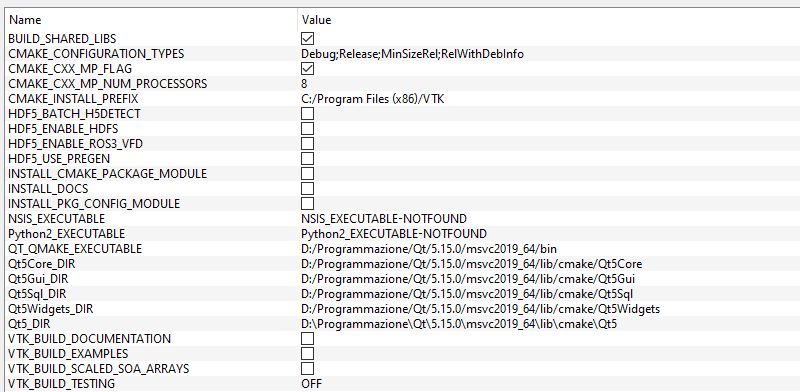
\includegraphics[width=1\textwidth]{immagini/svolgimento/vtkcmake.png}
    \caption{\textit{Alcuni parametri di configurazione di VTK su CMake-gui}}
    \textbf{Fonte}: Stage
    \label{fig: VTK CMAKE}
\end{figure}

A parte qualche dubbio nella compilazione tuttavia, VTK offre una ampia gamma di esempi, ed è stato quindi molto interessante ed utile analizzarne i principali per comprenderne il funzionamento e le basi. Oltre agli esempi ufficiali comunque, se ne trovano moltissimi anche su GitHub, grazie alla comunità.

\subsection{Primo CMakeLists}
Come menzionato nella sezione precedente, avevo esperienza nel fare la compilazione di alcune librerie utilizzando CMake, ma non lo avevo mai utilizzato in un progetto personale. Nel Piano di Lavoro CMake era segnato come obiettivo facoltativo con:"F03: porting librerie aziendali su CMake;". \'E stato invece deciso con il tutor di iniziare subito il progetto con CMake: innanzitutto per imparare come utilizzarlo e le basi, ma anche per non dover cambiare sistema di build in seguito.
\\
Qt utilizza di default un sistema di build basato su Makefile, generati tramite il comando proprietario qmake su un progetto ".pro". Questo funziona molto bene con Qt ma è specifico per l'utilizzo con Qt, CMake è un sistema di build molto più generico e ampiamente utilizzato. L'azienda voleva esplorarne le capacità e le funzionalità, e anche io ero molto interessato ad imparare come utilizzarlo meglio. CMake funziona tramite la scrittura di uno o più CMakeLists.txt, che definiscono tutti i parametri di configurazione del progetto, le librerie esterne, e i file da compilare. Per nostra fortuna Qt ha il supporto a CMake quindi non è complesso da integrare. Diamo un'occhiata ad un semplice CMakeLists.txt di base per Qt.

\begin{minted}{cmake}
cmake_minimum_required(VERSION 3.15.4)

project(helloworld)

set(CMAKE_AUTOMOC ON)
set(CMAKE_AUTORCC ON)

find_package(Qt5 COMPONENTS Widgets REQUIRED)

add_executable(helloworld
    mainwindow.ui
    mainwindow.cpp
    main.cpp
    resources.qrc
)

target_link_libraries(helloworld Qt5::Widgets)
\end{minted}


\subsection{Integrazione Qt-VTK}
\intro{Le prime prove nell'utilizzare VTK con Qt}\\

\subsection{Primo prototipo}
\intro{Il primo prototipo funzionante di visualizzatore}\\

\subsection{Aggiunta strumenti}
\intro{Gli strumenti aggiunti per interagire con il volume, tra cui Mark}\\

\subsection{Compilazione librerie aziendali}
\intro{Le librerie aziendali da utilizzare e i problemi nel compilarle}\\

\subsection{Problemi librerie aziendali}
\intro{I problemi nell'utilizzare le librerie aziendali con VTK}\\

\subsection{Modifiche interfaccia}
\intro{Com'è stata modificata l'interfaccia per renderla semplice e portatile}\\

%**************************************************************
\section{Documentazione}

%**************************************************************
\section{Test}
\subsection{Possibili test su una UI}
\intro{I problemi nel testare un'interfaccia grafica}\\

\subsection{Test di 3D Slicer e VTK}
\intro{Come 3D Slicer e VTK fanno questi test}\\

\subsection{Test implementati}
\intro{Discussione sui test fatti su librerie statiche e "model"}\\